Tübingen hat keine Universität, Tübingen \textbf{ist} eine Universität, daher existiert auch kein Uni-Campus im herkömmlichen Sinne. Alles spielt sich irgendwo in der Stadt ab, für euch im ersten Semester vor allem auf der Morgenstelle, später auch auf dem Sand. Damit ihr euch dort zurechtfindet, haben wir hier ein paar Lagepläne zusammengefasst. Diese sind keinesfalls allumfassend, sie sollen euch lediglich eine grobe Orientierung durch den Dschungel der Uni-Gebäude bieten.
\subsection*{Morgenstelle}
\begin{figure}[ht!]
\centering
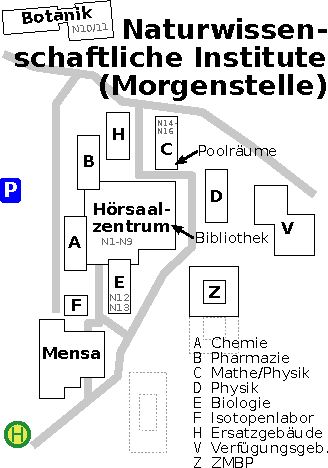
\includegraphics[width=0.5\textwidth]{info/anhang/lageplaene/uebersicht_morgenstelle.pdf}
\end{figure}
\newpage
\subsection*{Sand}
\begin{figure}[ht!]
	\centering
	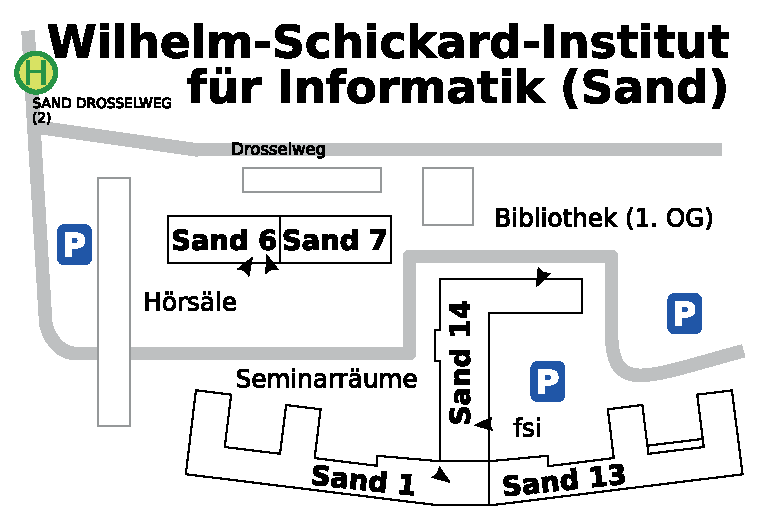
\includegraphics[width=0.8\textwidth]{info/anhang/lageplaene/uebersicht_sand.pdf}
\end{figure}
\subsubsection*{Sand, Erdgeschoss}~
\begin{figure}[ht!]
	\centering
	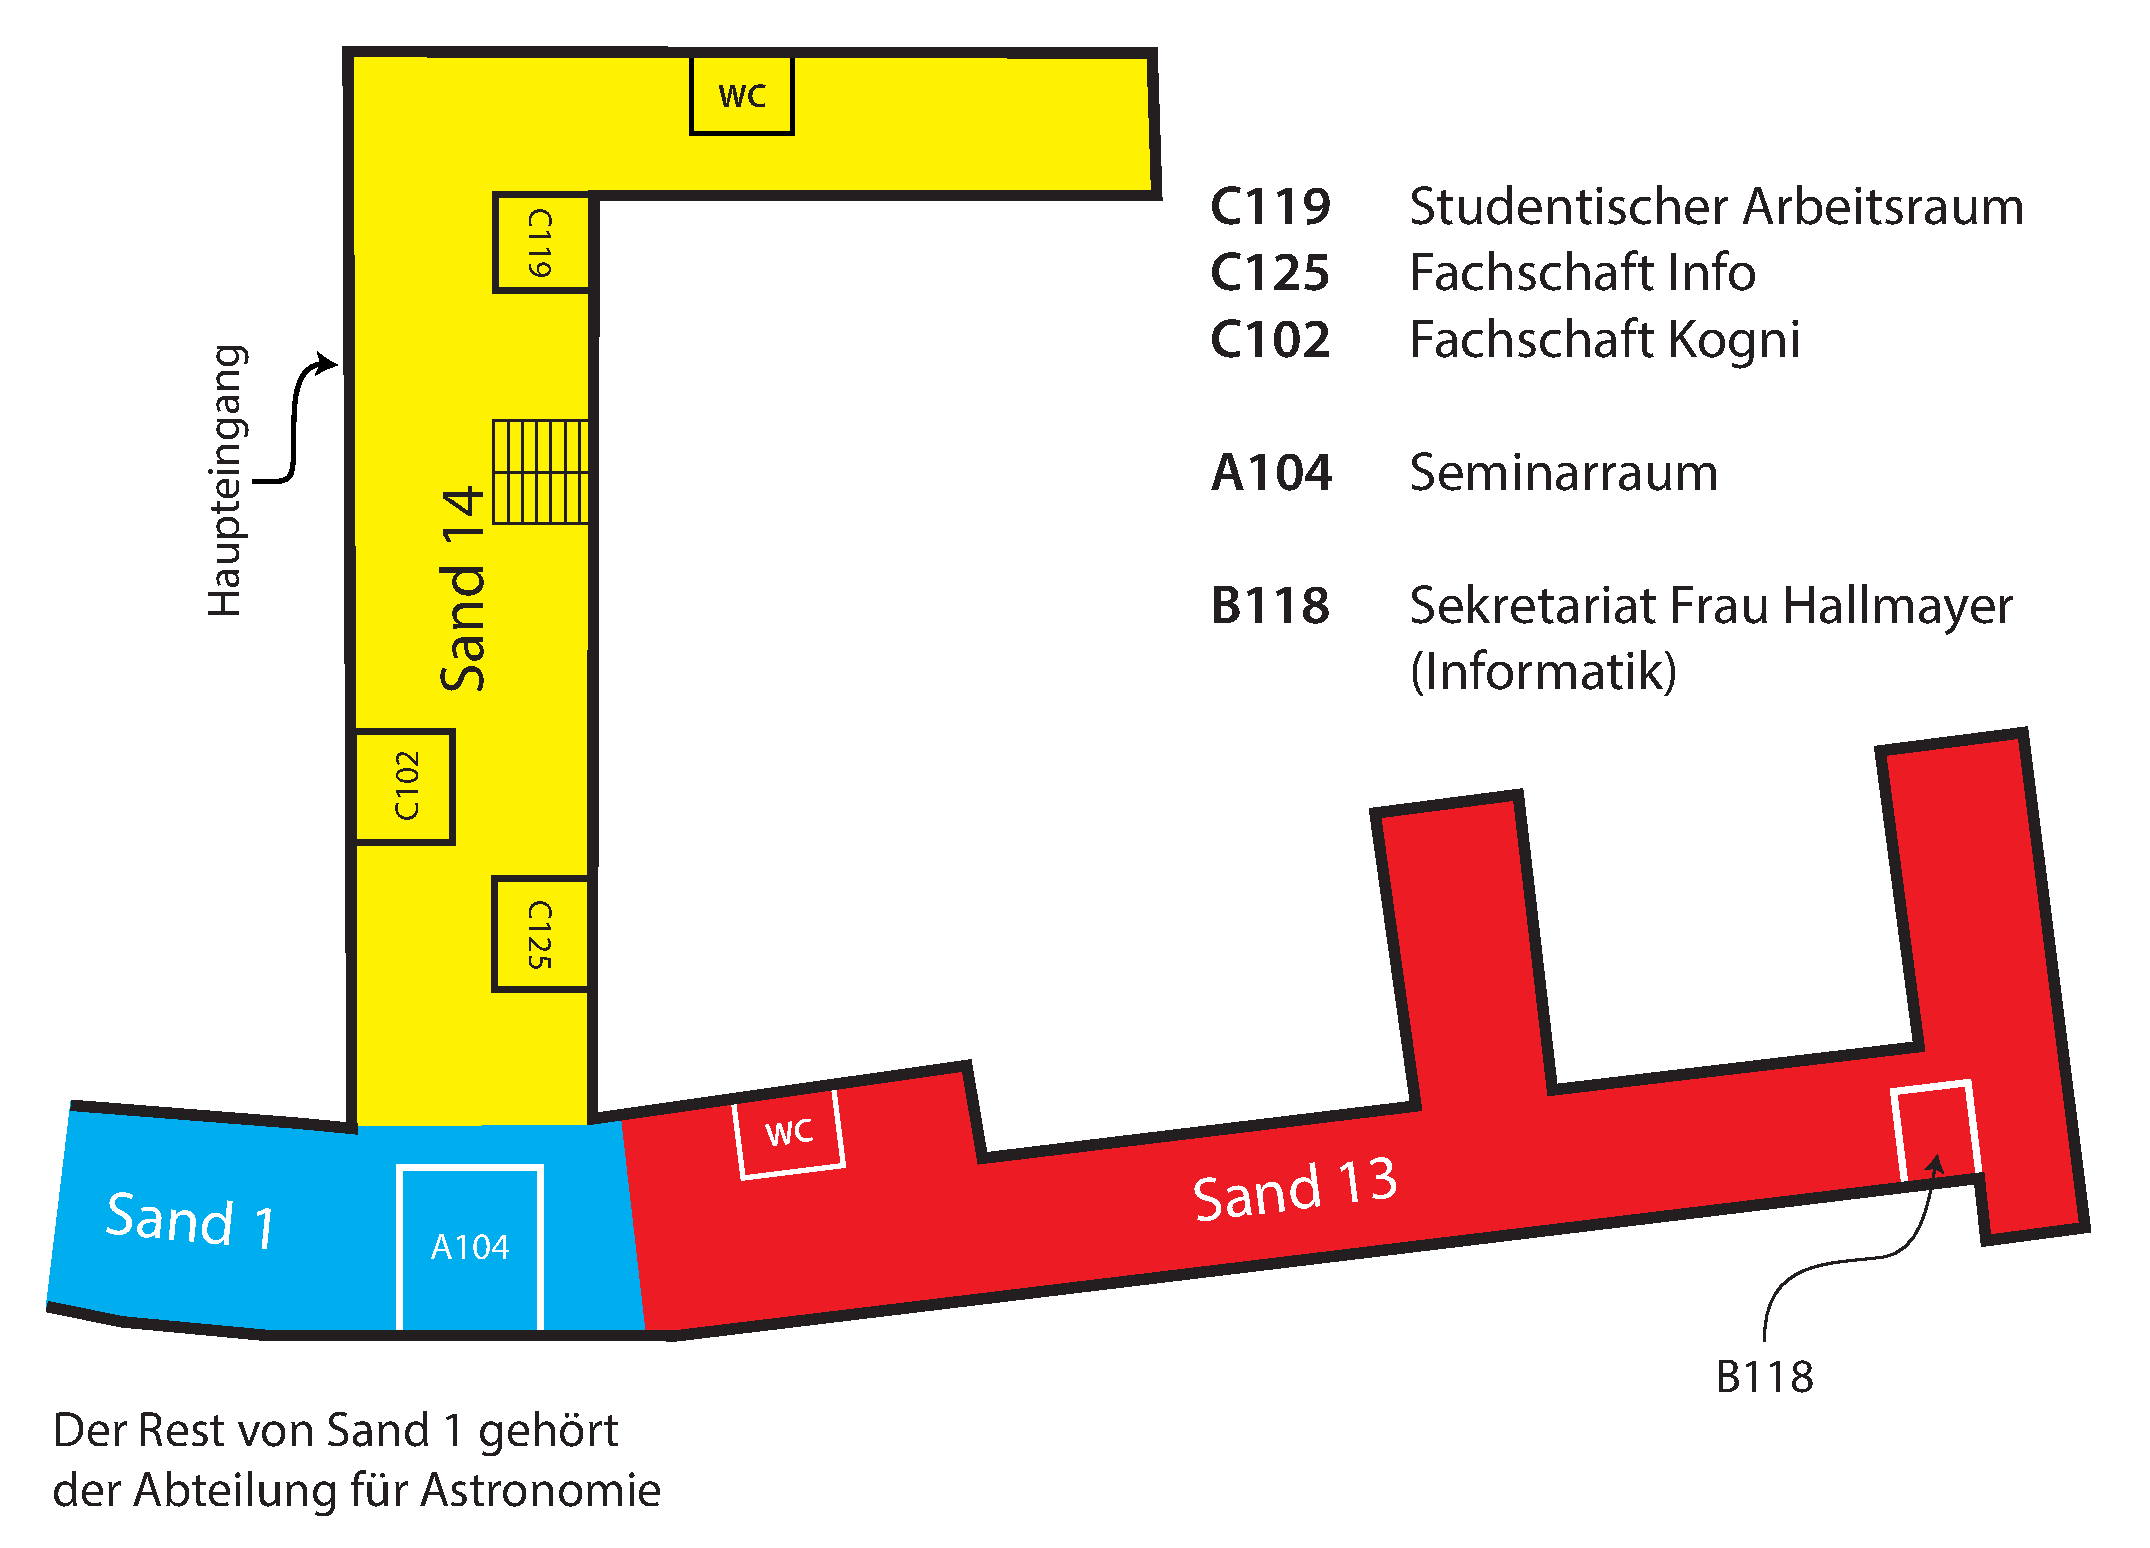
\includegraphics[width=0.9\textwidth]{info/anhang/lageplaene/sand_eg.pdf}
\end{figure}
\vfill 
\subsubsection*{Sand, 1. OG}~
\begin{figure}[ht!]
	\centering
	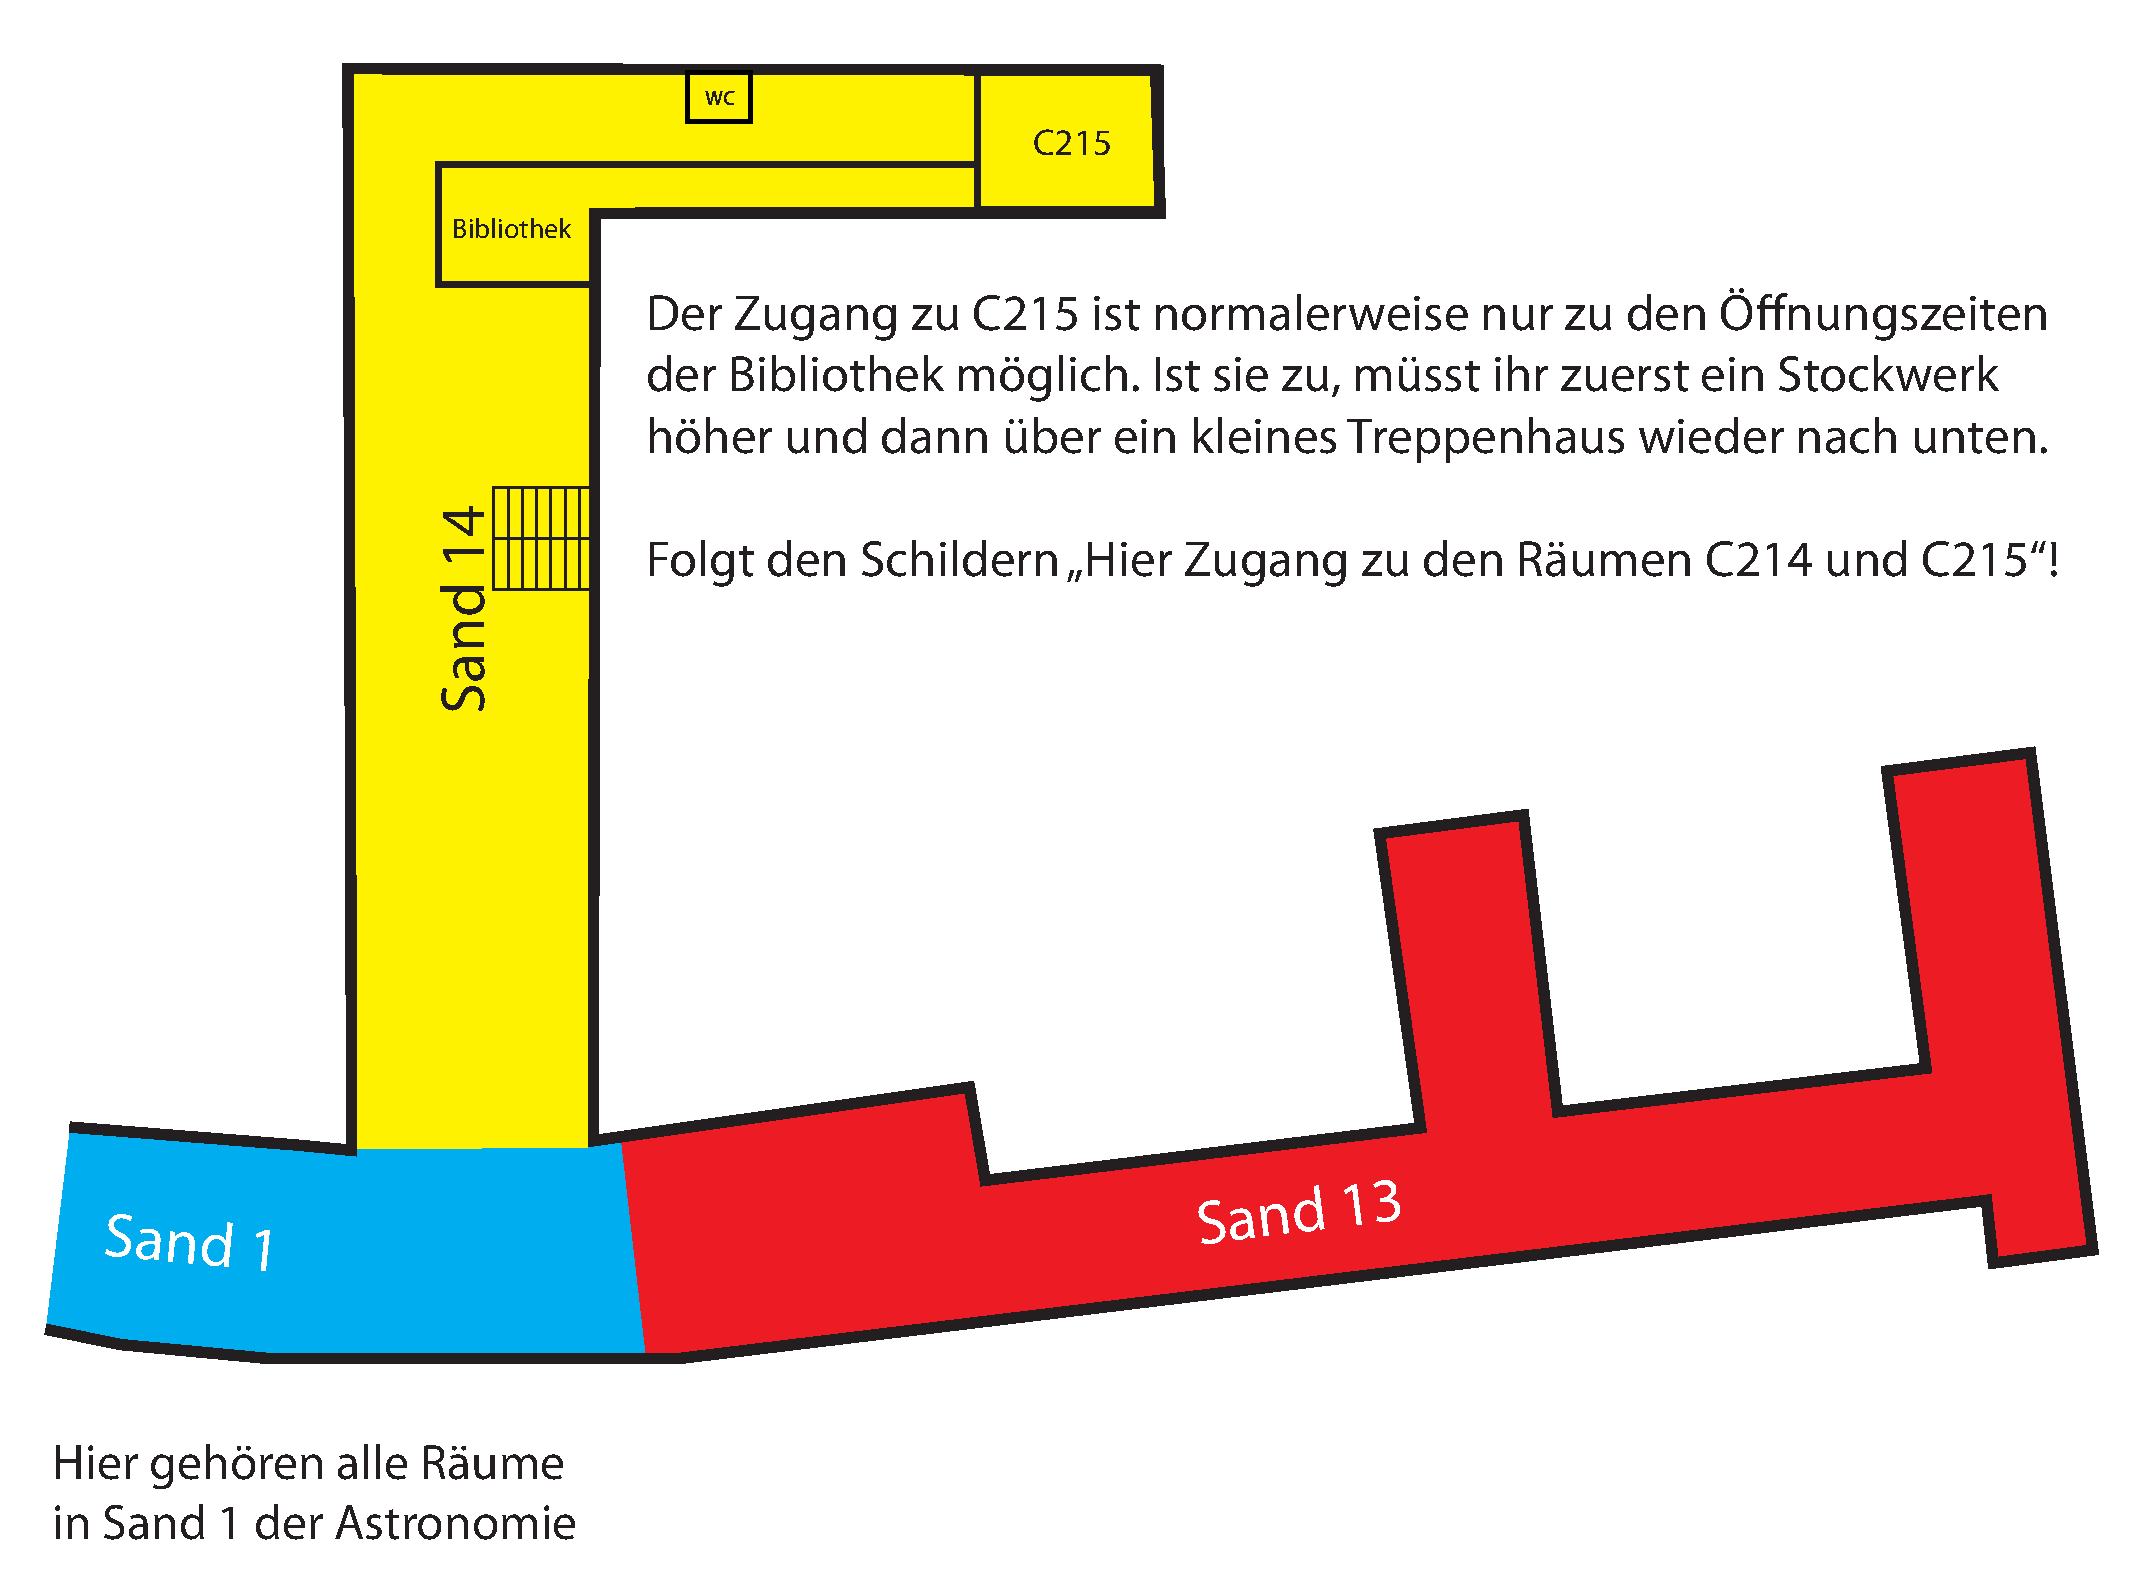
\includegraphics[width=0.9\textwidth]{info/anhang/lageplaene/sand_1og.pdf}
\end{figure}
\subsubsection*{Sand, 2. OG}~
\begin{figure}[ht!]
	\centering
	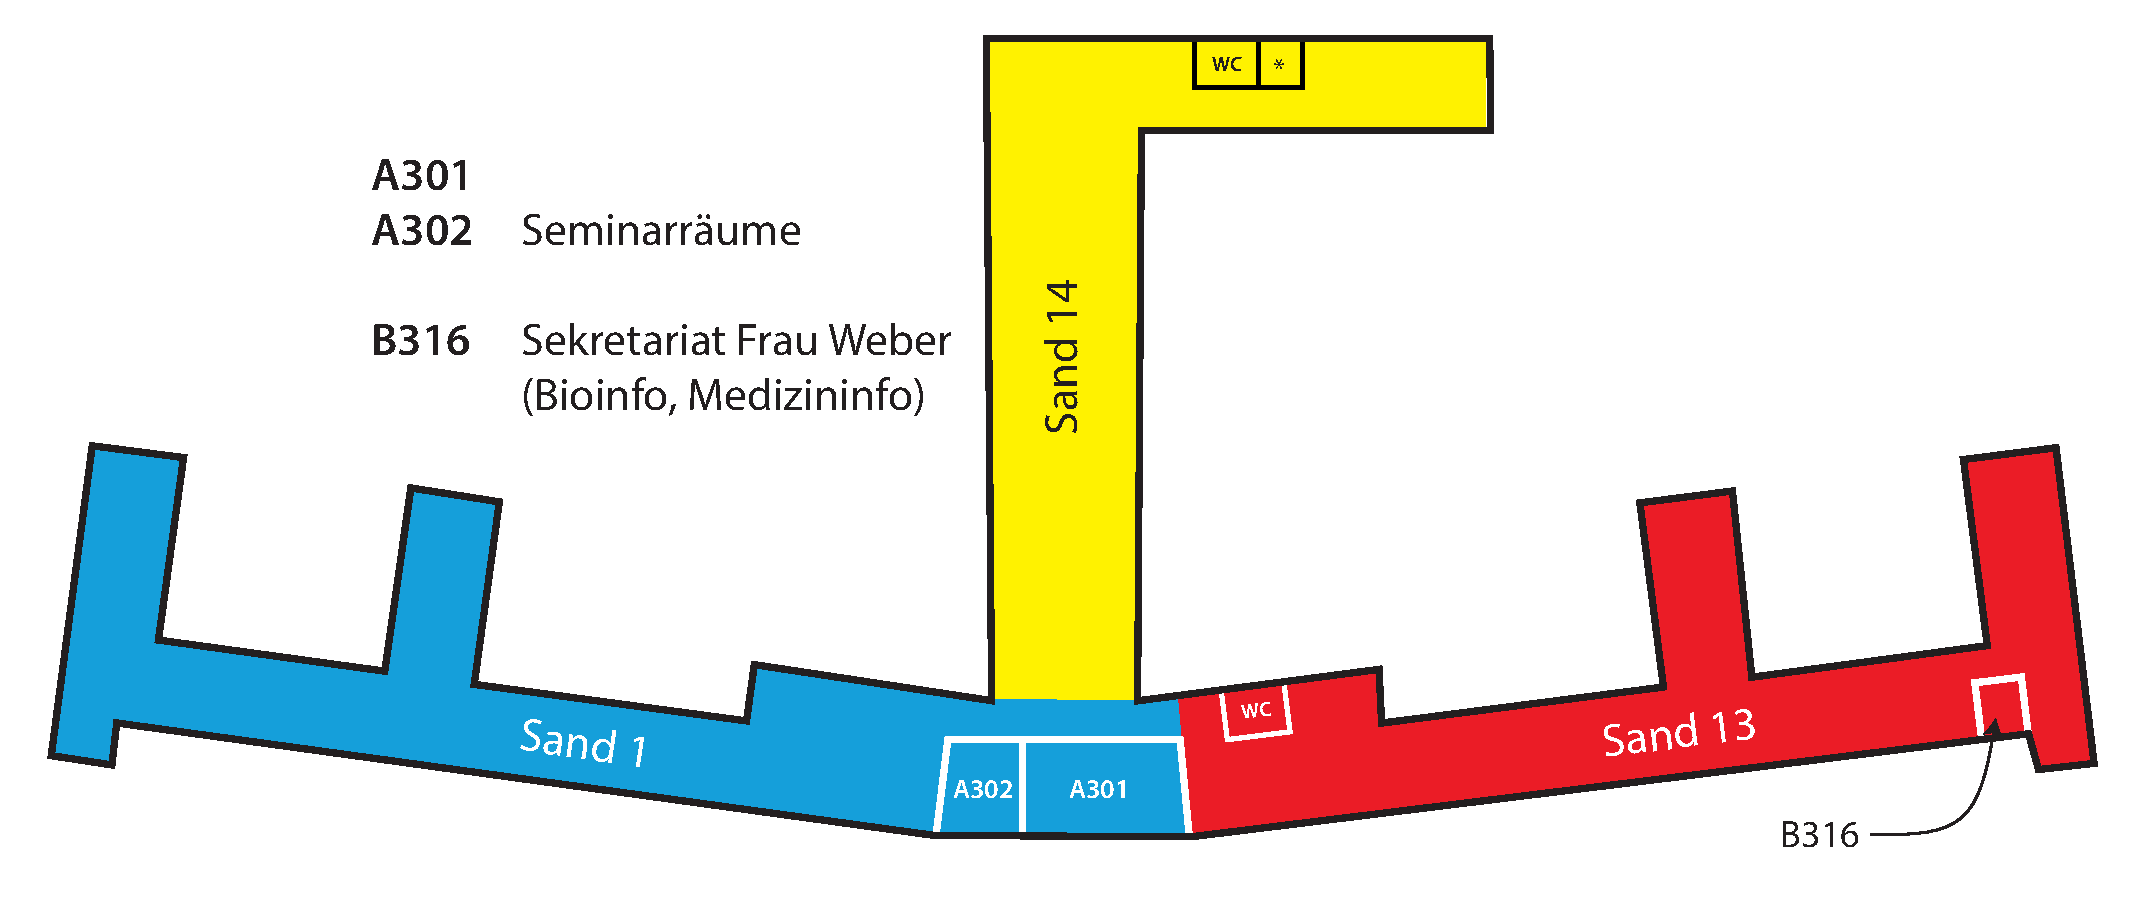
\includegraphics[width=\textwidth]{info/anhang/lageplaene/sand_2og.pdf}
\end{figure}